\section{Experiment E}

\begin{minipage}{0.45\textwidth}
	\centering
	\begin{tabular}{lr}
	\toprule
	\textbf{Hyperparameter} & \textbf{Value} \\
	\midrule
	Buffer Size & \\
	Batch Size & \\
	Gamma ($\gamma$) & \\
	Tau ($\tau$) & \\
	Actor Learning Rate & \\
	Critic Learning Rate & \\
	Weight Decay & \\
	OU Noise Mu ($\mu$) & \\
	OU Noise Theta ($\theta$) & \\
	OU Noise Mu ($\sigma$) & \\
	\bottomrule
	\end{tabular}
\end{minipage}
\hspace{1cm}
\begin{minipage}{0.45\textwidth}
	\centering
	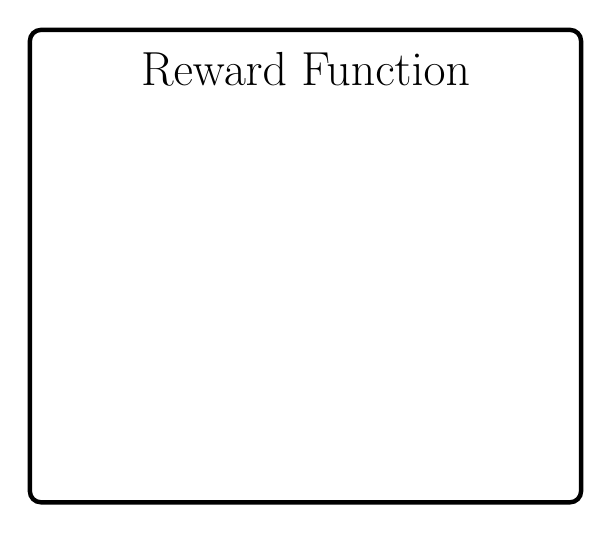
\begin{tikzpicture}
		\node (1) [draw, rectangle, minimum width=7cm, minimum height=6cm, rounded corners, ultra thick] {};
		\node at (0,2.5) {\LARGE Reward Function} ;
	\end{tikzpicture}
\end{minipage}

\begin{figure}[h]
	\begin{minipage}{0.45\textwidth}
		\centering
		% This file was created by tikzplotlib v0.9.1.
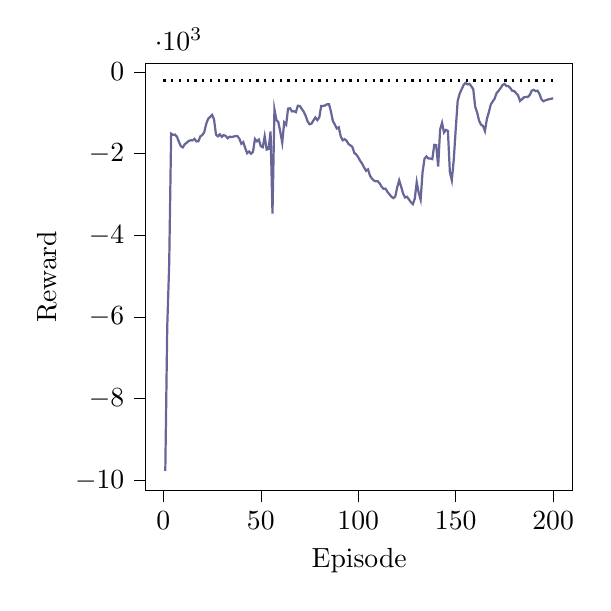
\begin{tikzpicture}

\definecolor{color0}{rgb}{0.12156862745098,0.466666666666667,0.705882352941177}

\begin{axis}[
compat=newest,
tick align=outside,
tick pos=left,
x grid style={white!69.0196078431373!black},
xmin=-8.95, xmax=209.95,
xtick style={color=black},
y grid style={white!69.0196078431373!black},
ymin=-10237.8868910548, ymax=203.619925054467,
ytick style={color=black},
scaled y ticks=true,
scaled y ticks=base 10:-3,
width=7cm,
height=7cm,
xlabel=Episode,
ylabel=Reward
]

\addplot[thick, black, dotted, domain=0:200] {-211.15};

\addplot [thick, blue!20!gray]
table {%
1 -9763.27294486799
2 -6233.80261025401
3 -4702.25607429109
4 -1512.21343297441
5 -1541.56062085325
6 -1535.22850284016
7 -1588.96606184897
8 -1715.23669898396
9 -1820.31231753912
10 -1847.66786072394
11 -1769.92450118555
12 -1734.64730574001
13 -1691.78106317152
14 -1674.45493906621
15 -1676.90591264538
16 -1640.75523295968
17 -1703.4048995174
18 -1697.83044713235
19 -1576.88921890067
20 -1546.5715732237
21 -1474.09512876949
22 -1271.65422689584
23 -1150.29854596291
24 -1102.56488295819
25 -1052.63460403206
26 -1160.0570975787
27 -1531.80428427574
28 -1577.96536228338
29 -1528.46964853933
30 -1588.81698896337
31 -1545.80968137986
32 -1568.85552000374
33 -1624.20152414619
34 -1586.50471460737
35 -1592.55986202214
36 -1584.94638344089
37 -1569.33361174512
38 -1573.1892994717
39 -1633.50494911412
40 -1759.32305467967
41 -1719.13862961987
42 -1862.97480239258
43 -1990.60310329712
44 -1948.10280201805
45 -2003.32412321478
46 -1956.29505058938
47 -1643.40355154487
48 -1699.32053231105
49 -1655.76163636967
50 -1820.85636906421
51 -1844.26667355161
52 -1574.87178814199
53 -1901.6723073915
54 -1886.04289052694
55 -1458.04140202327
56 -3469.32441220565
57 -917.195658586486
58 -1176.59257034398
59 -1230.33078309159
60 -1466.59633331869
61 -1732.22292637077
62 -1236.42594346941
63 -1293.97326214233
64 -899.857651460993
65 -890.845587246339
66 -968.24154739275
67 -963.199443956724
68 -986.677853906075
69 -828.526039545684
70 -834.720257437712
71 -902.709529703026
72 -972.62043534064
73 -1074.17044214855
74 -1209.87366623514
75 -1283.68681382054
76 -1267.54188154102
77 -1187.55869135607
78 -1114.1130550254
79 -1179.99960886007
80 -1115.99943619309
81 -832.657288986692
82 -832.72759717624
83 -822.279758669418
84 -793.164073797469
85 -791.044522604899
86 -972.019086460731
87 -1206.24867561322
88 -1290.02850233563
89 -1384.86591544101
90 -1357.00442247666
91 -1575.38270406248
92 -1674.08821396743
93 -1647.60414166174
94 -1684.15617335132
95 -1765.71695848599
96 -1797.33452011673
97 -1838.75461128161
98 -1985.76014825974
99 -2021.98376684527
100 -2092.02233018191
101 -2178.15994993705
102 -2247.02313410243
103 -2340.33340175948
104 -2420.7367742868
105 -2385.67777225085
106 -2538.2164437452
107 -2609.81411422946
108 -2659.40383450713
109 -2678.50832692135
110 -2676.82744132636
111 -2730.33624432342
112 -2812.33229768694
113 -2861.50305884707
114 -2857.37029123113
115 -2938.78510578548
116 -2994.46766053733
117 -3054.18167696401
118 -3089.68136986634
119 -3050.40051346782
120 -2823.26624003158
121 -2653.39029885552
122 -2806.59146922999
123 -2978.05949681073
124 -3075.60138846972
125 -3056.50890159285
126 -3119.86383000792
127 -3190.77697519937
128 -3237.45041767532
129 -3103.94340263226
130 -2698.75288944802
131 -2956.79624472601
132 -3124.84788885606
133 -2453.99592562811
134 -2125.61227356192
135 -2067.71562137431
136 -2118.05416804509
137 -2120.76157358531
138 -2134.78314728543
139 -1786.15300160098
140 -1793.00208055793
141 -2319.18931540986
142 -1413.05062097296
143 -1245.7107253682
144 -1484.37154592392
145 -1420.74714969691
146 -1446.61374769009
147 -2448.65824563979
148 -2652.9204998935
149 -2151.41685205676
150 -1409.62535384097
151 -715.425293566961
152 -537.233050162036
153 -429.756832729694
154 -325.6823376965
155 -270.994021132317
156 -306.189756950749
157 -292.000625606546
158 -350.489728088838
159 -423.619606641182
160 -855.467889009458
161 -994.472702683325
162 -1195.21463389004
163 -1292.79692031924
164 -1320.56851018644
165 -1448.16350042877
166 -1152.54457203662
167 -987.150718369486
168 -798.086323275897
169 -722.281160318246
170 -651.843048097534
171 -517.090294083444
172 -462.655401350926
173 -399.143888792889
174 -324.173287068825
175 -295.147502477148
176 -344.83352622425
177 -349.652649290451
178 -394.784026316548
179 -462.079584436464
180 -468.014634507583
181 -522.962154721305
182 -573.619728760075
183 -711.92181205646
184 -671.105200941416
185 -622.486488273209
186 -613.495902939192
187 -614.457292613144
188 -566.095980332205
189 -462.064404335876
190 -440.344339674872
191 -470.810273558386
192 -460.606507255502
193 -542.73700519533
194 -671.942780564072
195 -720.097164404344
196 -696.536841144416
197 -680.892791035771
198 -667.588830250088
199 -657.904337807085
200 -646.907259376791
};
\end{axis}

\end{tikzpicture}

		\caption{text}
		\label{fig:5501_raw_reward}
	\end{minipage}
	\hspace{0.75cm}
	\begin{minipage}{0.45\textwidth}
		\centering
		% This file was created by tikzplotlib v0.9.1.
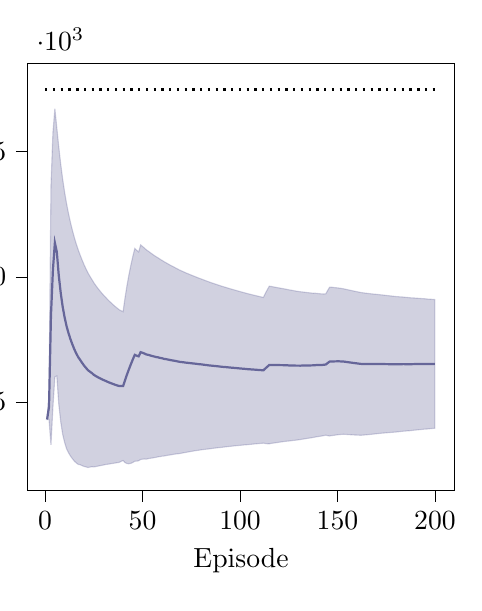
\begin{tikzpicture}[trim axis right,trim axis left]

\definecolor{color0}{rgb}{1,0.498039215686275,0.0549019607843137}
\definecolor{color1}{rgb}{0.12156862745098,0.466666666666667,0.705882352941177}

\begin{axis}[
compat=newest,
tick align=outside,
tick pos=left,
x grid style={white!69.0196078431373!black},
xmin=-8.95, xmax=209.95,
xtick style={color=black},
y grid style={white!69.0196078431373!black},
ymin=-8500, ymax=8500,
ytick style={color=black},
scaled y ticks=true,
scaled y ticks=base 10:-3,
width=7cm,
height=7cm,
xlabel=Episode,
ylabel=Average Reward,
y label style={at={(-0.2,0.5)}}
]

\addplot[thick, black, dotted, domain=0:200] {7461.75};

\path [draw=blue!20!gray, fill=blue!20!gray, opacity=0.3]
(axis cs:1,-5683.54889736257)
--(axis cs:1,-5683.54889736257)
--(axis cs:2,-4664.83596416343)
--(axis cs:3,3611.91015013816)
--(axis cs:4,5733.02874612919)
--(axis cs:5,6703.08679409963)
--(axis cs:6,5941.79779738927)
--(axis cs:7,5181.06295860306)
--(axis cs:8,4495.95947900039)
--(axis cs:9,3896.14664603212)
--(axis cs:10,3376.32312938225)
--(axis cs:11,2920.32294307545)
--(axis cs:12,2525.15744349306)
--(axis cs:13,2171.95496132655)
--(axis cs:14,1855.64226679598)
--(axis cs:15,1566.84923818866)
--(axis cs:16,1307.31486451035)
--(axis cs:17,1070.69485921444)
--(axis cs:18,865.172963604798)
--(axis cs:19,666.607874756861)
--(axis cs:20,482.804895974852)
--(axis cs:21,314.974734842627)
--(axis cs:22,155.659446332147)
--(axis cs:23,21.7160298397339)
--(axis cs:24,-103.627696733365)
--(axis cs:25,-233.036955279191)
--(axis cs:26,-344.647576742026)
--(axis cs:27,-448.279912845569)
--(axis cs:28,-547.517237316667)
--(axis cs:29,-640.829735566254)
--(axis cs:30,-729.086315506914)
--(axis cs:31,-811.631395319951)
--(axis cs:32,-894.282644343613)
--(axis cs:33,-972.142856413599)
--(axis cs:34,-1045.03321156417)
--(axis cs:35,-1116.03381064321)
--(axis cs:36,-1183.19899074506)
--(axis cs:37,-1247.5833211883)
--(axis cs:38,-1309.1740200345)
--(axis cs:39,-1348.94779476236)
--(axis cs:40,-1388.22143226712)
--(axis cs:41,-832.681807583704)
--(axis cs:42,-347.454624180522)
--(axis cs:43,84.0036460116467)
--(axis cs:44,468.613736115966)
--(axis cs:45,816.276437284182)
--(axis cs:46,1132.04168979841)
--(axis cs:47,1058.75280272605)
--(axis cs:48,993.078178500789)
--(axis cs:49,1275.22921923384)
--(axis cs:50,1209.90250609426)
--(axis cs:51,1144.43099871621)
--(axis cs:52,1074.28967068447)
--(axis cs:53,1021.84969181031)
--(axis cs:54,963.284822882199)
--(axis cs:55,906.122375984313)
--(axis cs:56,853.673190284089)
--(axis cs:57,800.474787773306)
--(axis cs:58,754.792361481015)
--(axis cs:59,702.052554214804)
--(axis cs:60,657.200702192931)
--(axis cs:61,605.777553627973)
--(axis cs:62,563.911623111233)
--(axis cs:63,519.849948570358)
--(axis cs:64,475.177789641657)
--(axis cs:65,433.392340412509)
--(axis cs:66,393.703789909052)
--(axis cs:67,353.560947382149)
--(axis cs:68,311.457997567784)
--(axis cs:69,271.135512767131)
--(axis cs:70,236.53417834949)
--(axis cs:71,202.336943876262)
--(axis cs:72,166.771237469463)
--(axis cs:73,134.735395726961)
--(axis cs:74,102.300119821232)
--(axis cs:75,70.5415149877558)
--(axis cs:76,38.8998242521016)
--(axis cs:77,8.97464552618476)
--(axis cs:78,-22.4708054821217)
--(axis cs:79,-53.7952376816515)
--(axis cs:80,-80.6679858663811)
--(axis cs:81,-111.032851575875)
--(axis cs:82,-140.763643927183)
--(axis cs:83,-169.462762129693)
--(axis cs:84,-198.893047108781)
--(axis cs:85,-225.692446338669)
--(axis cs:86,-251.539196494657)
--(axis cs:87,-277.924552937011)
--(axis cs:88,-303.697000827866)
--(axis cs:89,-329.330756837966)
--(axis cs:90,-356.111224723384)
--(axis cs:91,-381.184714059792)
--(axis cs:92,-404.195999696266)
--(axis cs:93,-427.303858793827)
--(axis cs:94,-451.384865611832)
--(axis cs:95,-475.032255001821)
--(axis cs:96,-497.603548377329)
--(axis cs:97,-519.211771923848)
--(axis cs:98,-541.272582843804)
--(axis cs:99,-563.88105569437)
--(axis cs:100,-585.761721153127)
--(axis cs:101,-607.311927425352)
--(axis cs:102,-627.865031243257)
--(axis cs:103,-649.029039005381)
--(axis cs:104,-670.628274582017)
--(axis cs:105,-689.617138377228)
--(axis cs:106,-709.454379164859)
--(axis cs:107,-727.434389108195)
--(axis cs:108,-746.343417065776)
--(axis cs:109,-765.797160678988)
--(axis cs:110,-783.92941074887)
--(axis cs:111,-802.540185305784)
--(axis cs:112,-820.012485104501)
--(axis cs:113,-659.491904486838)
--(axis cs:114,-510.765947503894)
--(axis cs:115,-372.25379264869)
--(axis cs:116,-381.63466107484)
--(axis cs:117,-397.349084447256)
--(axis cs:118,-412.622872398521)
--(axis cs:119,-427.400565002773)
--(axis cs:120,-440.726717489241)
--(axis cs:121,-455.248878102756)
--(axis cs:122,-468.418119542088)
--(axis cs:123,-482.312957038475)
--(axis cs:124,-498.190120384759)
--(axis cs:125,-514.94702411482)
--(axis cs:126,-528.852569547214)
--(axis cs:127,-540.735496322354)
--(axis cs:128,-556.814386191515)
--(axis cs:129,-570.14102094993)
--(axis cs:130,-581.782359374813)
--(axis cs:131,-593.653350383089)
--(axis cs:132,-601.515781135316)
--(axis cs:133,-611.93166274735)
--(axis cs:134,-621.185156621406)
--(axis cs:135,-629.964309509482)
--(axis cs:136,-638.978312806904)
--(axis cs:137,-646.942638411365)
--(axis cs:138,-654.030553328018)
--(axis cs:139,-655.270481440334)
--(axis cs:140,-664.044182267109)
--(axis cs:141,-672.627365453917)
--(axis cs:142,-679.264226520177)
--(axis cs:143,-682.270853033164)
--(axis cs:144,-676.179609271668)
--(axis cs:145,-535.532678327405)
--(axis cs:146,-409.10703793009)
--(axis cs:147,-411.892717803471)
--(axis cs:148,-421.886643796738)
--(axis cs:149,-431.226425078718)
--(axis cs:150,-438.443559640129)
--(axis cs:151,-448.832961296134)
--(axis cs:152,-462.111885336255)
--(axis cs:153,-473.787502508091)
--(axis cs:154,-491.074439689155)
--(axis cs:155,-508.178273268498)
--(axis cs:156,-525.262251102121)
--(axis cs:157,-542.114177466339)
--(axis cs:158,-558.757150489942)
--(axis cs:159,-575.441355335804)
--(axis cs:160,-591.219066137176)
--(axis cs:161,-607.478431196642)
--(axis cs:162,-623.235129955506)
--(axis cs:163,-634.297692200927)
--(axis cs:164,-644.480211434214)
--(axis cs:165,-654.838603405442)
--(axis cs:166,-664.336515971049)
--(axis cs:167,-673.141378223671)
--(axis cs:168,-681.64023579622)
--(axis cs:169,-689.371401014109)
--(axis cs:170,-696.51852122298)
--(axis cs:171,-704.579847351806)
--(axis cs:172,-713.629995994865)
--(axis cs:173,-720.566250020872)
--(axis cs:174,-730.592991023546)
--(axis cs:175,-739.593965263798)
--(axis cs:176,-748.328739205127)
--(axis cs:177,-757.657768142544)
--(axis cs:178,-765.901430865686)
--(axis cs:179,-775.238276040316)
--(axis cs:180,-784.236613202675)
--(axis cs:181,-788.032398170048)
--(axis cs:182,-796.338073103468)
--(axis cs:183,-800.698000145452)
--(axis cs:184,-806.647400905351)
--(axis cs:185,-816.081002827058)
--(axis cs:186,-821.283551232236)
--(axis cs:187,-831.564888999785)
--(axis cs:188,-835.926141988585)
--(axis cs:189,-840.501082580734)
--(axis cs:190,-846.117333717732)
--(axis cs:191,-852.141169682139)
--(axis cs:192,-858.157500729644)
--(axis cs:193,-863.358082117168)
--(axis cs:194,-868.356494583156)
--(axis cs:195,-873.984279746447)
--(axis cs:196,-883.081813687953)
--(axis cs:197,-888.312714201666)
--(axis cs:198,-892.506220919131)
--(axis cs:199,-898.528782160382)
--(axis cs:200,-904.170436091782)
--(axis cs:200,-6031.2460878229)
--(axis cs:200,-6031.2460878229)
--(axis cs:199,-6038.42444692848)
--(axis cs:198,-6045.34935076301)
--(axis cs:197,-6053.86032906361)
--(axis cs:196,-6061.66416558238)
--(axis cs:195,-6065.25582391111)
--(axis cs:194,-6072.91323682603)
--(axis cs:193,-6081.18190232796)
--(axis cs:192,-6089.38541297974)
--(axis cs:191,-6096.99883143657)
--(axis cs:190,-6104.70758222658)
--(axis cs:189,-6112.86796704833)
--(axis cs:188,-6121.93581697468)
--(axis cs:187,-6131.25369105158)
--(axis cs:186,-6134.27128768015)
--(axis cs:185,-6143.17027873174)
--(axis cs:184,-6147.79184367287)
--(axis cs:183,-6156.30310945593)
--(axis cs:182,-6166.12744810052)
--(axis cs:181,-6172.57677505633)
--(axis cs:180,-6182.98453626462)
--(axis cs:179,-6188.88606563874)
--(axis cs:178,-6194.5071756154)
--(axis cs:177,-6201.55352193547)
--(axis cs:176,-6207.4805834666)
--(axis cs:175,-6214.25969044175)
--(axis cs:174,-6220.87745823931)
--(axis cs:173,-6226.37102020022)
--(axis cs:172,-6235.35136223451)
--(axis cs:171,-6242.35822580188)
--(axis cs:170,-6250.56029605835)
--(axis cs:169,-6259.75692027889)
--(axis cs:168,-6268.56223540058)
--(axis cs:167,-6276.76440349625)
--(axis cs:166,-6284.80387771434)
--(axis cs:165,-6292.24997362599)
--(axis cs:164,-6298.8461803169)
--(axis cs:163,-6305.83428797796)
--(axis cs:162,-6311.89046479758)
--(axis cs:161,-6308.64551633529)
--(axis cs:160,-6304.04817807093)
--(axis cs:159,-6301.53490303241)
--(axis cs:158,-6296.27292900861)
--(axis cs:157,-6291.68075968238)
--(axis cs:156,-6286.79003510748)
--(axis cs:155,-6281.50617367602)
--(axis cs:154,-6276.67519043349)
--(axis cs:153,-6271.66681175566)
--(axis cs:152,-6278.75514946603)
--(axis cs:151,-6283.82778001546)
--(axis cs:150,-6292.83128193421)
--(axis cs:149,-6304.92343835404)
--(axis cs:148,-6315.3781087436)
--(axis cs:147,-6325.39608866533)
--(axis cs:146,-6340.84189458265)
--(axis cs:145,-6327.81831465658)
--(axis cs:144,-6306.89965939055)
--(axis cs:143,-6325.11253435764)
--(axis cs:142,-6340.12110683673)
--(axis cs:141,-6353.03092173095)
--(axis cs:140,-6364.58932305702)
--(axis cs:139,-6376.18686354583)
--(axis cs:138,-6392.78251792671)
--(axis cs:137,-6406.13126575647)
--(axis cs:136,-6419.01486662332)
--(axis cs:135,-6431.24748109409)
--(axis cs:134,-6443.90069010564)
--(axis cs:133,-6456.37703998253)
--(axis cs:132,-6468.03981521112)
--(axis cs:131,-6482.09614135046)
--(axis cs:130,-6492.81490908434)
--(axis cs:129,-6504.03840721376)
--(axis cs:128,-6513.70056482159)
--(axis cs:127,-6520.0055803875)
--(axis cs:126,-6531.80294640624)
--(axis cs:125,-6541.69280337811)
--(axis cs:124,-6548.07710001903)
--(axis cs:123,-6556.11608684203)
--(axis cs:122,-6566.96982103314)
--(axis cs:121,-6578.9349093524)
--(axis cs:120,-6589.7391700177)
--(axis cs:119,-6602.18766875233)
--(axis cs:118,-6613.39694392849)
--(axis cs:117,-6624.39238233312)
--(axis cs:116,-6635.23944676604)
--(axis cs:115,-6652.42655535755)
--(axis cs:114,-6649.23260596928)
--(axis cs:113,-6640.67278843788)
--(axis cs:112,-6625.56789396718)
--(axis cs:111,-6633.27170914044)
--(axis cs:110,-6639.69718238966)
--(axis cs:109,-6647.33515888778)
--(axis cs:108,-6653.39246063888)
--(axis cs:107,-6660.82335345178)
--(axis cs:106,-6670.08278996275)
--(axis cs:105,-6677.10981739834)
--(axis cs:104,-6685.93694360195)
--(axis cs:103,-6691.16018034103)
--(axis cs:102,-6697.73713484392)
--(axis cs:101,-6705.86872189792)
--(axis cs:100,-6713.02905834833)
--(axis cs:99,-6720.27792167371)
--(axis cs:98,-6726.97403151993)
--(axis cs:97,-6735.21010057888)
--(axis cs:96,-6744.76523516962)
--(axis cs:95,-6753.53065594397)
--(axis cs:94,-6761.29159862002)
--(axis cs:93,-6769.07621631272)
--(axis cs:92,-6779.09104988975)
--(axis cs:91,-6789.9512747808)
--(axis cs:90,-6798.44178336265)
--(axis cs:89,-6804.87733266241)
--(axis cs:88,-6814.08954486904)
--(axis cs:87,-6823.91767363679)
--(axis cs:86,-6833.64730044682)
--(axis cs:85,-6845.0505844711)
--(axis cs:84,-6855.9145518629)
--(axis cs:83,-6863.46326975569)
--(axis cs:82,-6873.25406853956)
--(axis cs:81,-6882.38557769733)
--(axis cs:80,-6891.5340948193)
--(axis cs:79,-6906.85348314655)
--(axis cs:78,-6916.66883780809)
--(axis cs:77,-6927.44482921364)
--(axis cs:76,-6941.64037869985)
--(axis cs:75,-6954.46684421078)
--(axis cs:74,-6968.31389871547)
--(axis cs:73,-6982.39086047354)
--(axis cs:72,-6998.28127661371)
--(axis cs:71,-7010.20884917465)
--(axis cs:70,-7025.62260861678)
--(axis cs:69,-7041.83872919554)
--(axis cs:68,-7050.35145953409)
--(axis cs:67,-7057.32399564148)
--(axis cs:66,-7069.63771716767)
--(axis cs:65,-7084.41731355485)
--(axis cs:64,-7097.63554062878)
--(axis cs:63,-7107.84849873977)
--(axis cs:62,-7121.18631107269)
--(axis cs:61,-7139.91462246515)
--(axis cs:60,-7144.0255651109)
--(axis cs:59,-7162.31748977068)
--(axis cs:58,-7169.29010654207)
--(axis cs:57,-7190.6723039468)
--(axis cs:56,-7202.43653618954)
--(axis cs:55,-7218.27733110353)
--(axis cs:54,-7228.64953833879)
--(axis cs:53,-7239.59974889705)
--(axis cs:52,-7263.65891887062)
--(axis cs:51,-7256.29345893705)
--(axis cs:50,-7264.57864669187)
--(axis cs:49,-7277.16130265562)
--(axis cs:48,-7327.87082996043)
--(axis cs:47,-7342.93830091869)
--(axis cs:46,-7347.33946452446)
--(axis cs:45,-7394.94018115896)
--(axis cs:44,-7429.54005565069)
--(axis cs:43,-7447.04917501062)
--(axis cs:42,-7440.34838948662)
--(axis cs:41,-7401.85840096014)
--(axis cs:40,-7316.98700665912)
--(axis cs:39,-7353.21111345835)
--(axis cs:38,-7391.92416537074)
--(axis cs:37,-7404.60810131042)
--(axis cs:36,-7417.19550584388)
--(axis cs:35,-7430.06008307852)
--(axis cs:34,-7441.56207713774)
--(axis cs:33,-7455.87504405004)
--(axis cs:32,-7467.56084618186)
--(axis cs:31,-7477.36193897716)
--(axis cs:30,-7495.50826016806)
--(axis cs:29,-7511.54938082628)
--(axis cs:28,-7527.39702695349)
--(axis cs:27,-7542.17888865599)
--(axis cs:26,-7559.87657914347)
--(axis cs:25,-7574.52714205937)
--(axis cs:24,-7563.55722867932)
--(axis cs:23,-7579.94236047905)
--(axis cs:22,-7596.39190182731)
--(axis cs:21,-7573.17902742429)
--(axis cs:20,-7555.14793935344)
--(axis cs:19,-7523.8724538693)
--(axis cs:18,-7486.8550601675)
--(axis cs:17,-7472.85782177765)
--(axis cs:16,-7415.18046242757)
--(axis cs:15,-7344.11905413163)
--(axis cs:14,-7244.7470402469)
--(axis cs:13,-7138.98036628439)
--(axis cs:12,-7006.33538618331)
--(axis cs:11,-6849.89509398383)
--(axis cs:10,-6598.79408408633)
--(axis cs:9,-6272.00834691501)
--(axis cs:8,-5768.96148369249)
--(axis cs:7,-5063.03387118719)
--(axis cs:6,-3948.90904773556)
--(axis cs:5,-3985.04937100994)
--(axis cs:4,-5186.08579412095)
--(axis cs:3,-6695.57327412097)
--(axis cs:2,-5683.54889736257)
--(axis cs:1,-5683.54889736257)
--cycle;

\addplot [thick, blue!20!gray]
table {%
1 -5683.54889736257
2 -5174.192430763
3 -1541.8315619914
4 273.471476004121
5 1359.01871154484
6 996.444374826857
7 59.0145437079384
8 -636.501002346052
9 -1187.93085044144
10 -1611.23547735204
11 -1964.78607545419
12 -2240.58897134512
13 -2483.51270247892
14 -2694.55238672546
15 -2888.63490797148
16 -3053.93279895861
17 -3201.0814812816
18 -3310.84104828135
19 -3428.63228955622
20 -3536.17152168929
21 -3629.10214629083
22 -3720.36622774758
23 -3779.11316531966
24 -3833.59246270634
25 -3903.78204866928
26 -3952.26207794275
27 -3995.22940075078
28 -4037.45713213508
29 -4076.18955819627
30 -4112.29728783748
31 -4144.49666714855
32 -4180.92174526274
33 -4214.00895023182
34 -4243.29764435096
35 -4273.04694686086
36 -4300.19724829447
37 -4326.09571124936
38 -4350.54909270262
39 -4351.07945411036
40 -4352.60421946312
41 -4117.27010427192
42 -3893.90150683357
43 -3681.52276449949
44 -3480.46315976736
45 -3289.33187193739
46 -3107.64888736302
47 -3142.09274909632
48 -3167.39632572982
49 -3000.96604171089
50 -3027.33807029881
51 -3055.93123011042
52 -3094.68462409308
53 -3108.87502854337
54 -3132.6823577283
55 -3156.07747755961
56 -3174.38167295272
57 -3195.09875808675
58 -3207.24887253053
59 -3230.13246777794
60 -3243.41243145899
61 -3267.06853441859
62 -3278.63734398073
63 -3293.9992750847
64 -3311.22887549356
65 -3325.51248657117
66 -3337.96696362931
67 -3351.88152412967
68 -3369.44673098315
69 -3385.3516082142
70 -3394.54421513364
71 -3403.93595264919
72 -3415.75501957212
73 -3423.82773237329
74 -3433.00688944712
75 -3441.96266461151
76 -3451.37027722388
77 -3459.23509184373
78 -3469.56982164511
79 -3480.3243604141
80 -3486.10104034284
81 -3496.7092146366
82 -3507.00885623337
83 -3516.46301594269
84 -3527.40379948584
85 -3535.37151540488
86 -3542.59324847074
87 -3550.9211132869
88 -3558.89327284846
89 -3567.10404475019
90 -3577.27650404302
91 -3585.5679944203
92 -3591.64352479301
93 -3598.19003755328
94 -3606.33823211593
95 -3614.28145547289
96 -3621.18439177348
97 -3627.21093625136
98 -3634.12330718187
99 -3642.07948868404
100 -3649.39538975073
101 -3656.59032466163
102 -3662.80108304359
103 -3670.09460967321
104 -3678.28260909198
105 -3683.36347788778
106 -3689.7685845638
107 -3694.12887127999
108 -3699.86793885233
109 -3706.56615978338
110 -3711.81329656927
111 -3717.90594722311
112 -3722.79018953584
113 -3650.08234646236
114 -3579.99927673659
115 -3512.34017400312
116 -3508.43705392044
117 -3510.87073339019
118 -3513.00990816351
119 -3514.79411687755
120 -3515.23294375347
121 -3517.09189372758
122 -3517.69397028762
123 -3519.21452194025
124 -3523.13361020189
125 -3528.31991374646
126 -3530.32775797673
127 -3530.37053835493
128 -3535.25747550656
129 -3537.08971408184
130 -3537.29863422958
131 -3537.87474586678
132 -3534.77779817322
133 -3534.15435136494
134 -3532.54292336352
135 -3530.60589530179
136 -3528.99658971511
137 -3526.53695208392
138 -3523.40653562737
139 -3515.72867249308
140 -3514.31675266206
141 -3512.82914359243
142 -3509.69266667845
143 -3503.6916936954
144 -3491.53963433111
145 -3431.67549649199
146 -3374.97446625637
147 -3368.6444032344
148 -3368.63237627017
149 -3368.07493171638
150 -3365.63742078717
151 -3366.3303706558
152 -3370.43351740114
153 -3372.72715713188
154 -3383.87481506132
155 -3394.84222347226
156 -3406.0261431048
157 -3416.89746857436
158 -3427.51503974928
159 -3438.48812918411
160 -3447.63362210405
161 -3458.06197376597
162 -3467.56279737654
163 -3470.06599008944
164 -3471.66319587556
165 -3473.54428851571
166 -3474.57019684269
167 -3474.95289085996
168 -3475.1012355984
169 -3474.5641606465
170 -3473.53940864066
171 -3473.46903657684
172 -3474.49067911469
173 -3473.46863511054
174 -3475.73522463143
175 -3476.92682785278
176 -3477.90466133586
177 -3479.60564503901
178 -3480.20430324054
179 -3482.06217083953
180 -3483.61057473365
181 -3480.30458661319
182 -3481.23276060199
183 -3478.50055480069
184 -3477.21962228911
185 -3479.6256407794
186 -3477.77741945619
187 -3481.40929002568
188 -3478.93097948163
189 -3476.68452481453
190 -3475.41245797215
191 -3474.57000055935
192 -3473.77145685469
193 -3472.26999222257
194 -3470.6348657046
195 -3469.62005182878
196 -3472.37298963517
197 -3471.08652163264
198 -3468.92778584107
199 -3468.47661454443
200 -3467.70826195734
};
\end{axis}

\end{tikzpicture}

		\caption{text}
		\label{fig:5502_average_reward}
	\end{minipage}
\end{figure}

\begin{figure}[h]
	\begin{minipage}{0.45\textwidth}
		\centering
		%\input{file_path}
		\caption{text}
		\label{key}
	\end{minipage}
	\hspace{1cm}
	\begin{minipage}{0.45\textwidth}
		\centering
		%\input{file_path}
		\caption{text}
		\label{key}
	\end{minipage}
\end{figure}

\begin{figure}[h]
	\begin{minipage}{0.45\textwidth}
		\centering
		%\input{file_path}
		\caption{text}
		\label{key}
	\end{minipage}
	\hspace{1cm}
	\begin{minipage}{0.45\textwidth}
		\centering
		%\input{file_path}
		\caption{text}
		\label{key}
	\end{minipage}
\end{figure}